
\documentclass[10pt]{article}

\usepackage[T1]{fontenc}
\usepackage[utf8]{inputenc}

\usepackage{MinionPro}

\usepackage{graphicx}
\usepackage[unicode,linktocpage]{hyperref}
\hypersetup{
    colorlinks=true,
    pdfpagelayout=SinglePage,
    pdfpagemode=UseOutlines,
    pdfstartview=Fit,
    linkcolor=black,
    citecolor=black,
    anchorcolor=black,
    filecolor=black,
    menucolor=black,
    pagecolor=black,
    urlcolor=black,
    pdftitle={},
    pdfauthor={Dawid Weiss},
    pdfkeywords={}
}
\usepackage{url}

\title{Legal Eye-candy fonts for \LaTeX{}?}
\author{Dawid Weiss}

\begin{document}

\maketitle%

\section{Introduction}

The default \LaTeX{} font is Computer Modern, designed by prof.~Donald Knuth himself. I like
it, but I've always been fond of two fonts from the Adobe font foundry -- Minion and Myriad.
Both typefaces were designed by Robert Slimbach and are available in numerous optical sizes
and variations. Unfortunately, as you might have guessed, not for free.

Recently, I've found out that Adobe added four standard (roman, oblique, bold and bold oblique)
Myriad and Minion font faces to a piece of freely available software -- 
Adobe Acrobat Reader, version 7.0. This is my log of actions to find out if this is really 
true and how to use these fonts with \LaTeX{}.

\section{Getting the fonts}

\begin{itemize}
    \item I downloaded Adobe Acrobat Reader from Adobe and installed it on my system. Looking
    at the installation folder reveals that, indeed, OpenType versions of
    Minion and Myriad are in:
    \begin{center}
    \textsf{c:$\backslash$Program Files$\backslash$Adobe$\backslash$Acrobat 7.0$\backslash$Resource}
    \end{center}
    
    \item In the first step, I'll just copy OpenType fonts to my Windows fonts folder,
    permitting me to use Minion in OpenOffice. It works on display (and looks really ugly, as if
    not font smoothing have been applied), plus I couldn't embed the fonts in an 
    exported \texttt{pdf}. A workaround is to use a postscript printer and convert
    the \texttt{ps} file to \texttt{pdf} manually -- results
    in Figure~\ref{fig:openoffice}.
\end{itemize}

\begin{figure}[p]
\centering%
\fbox{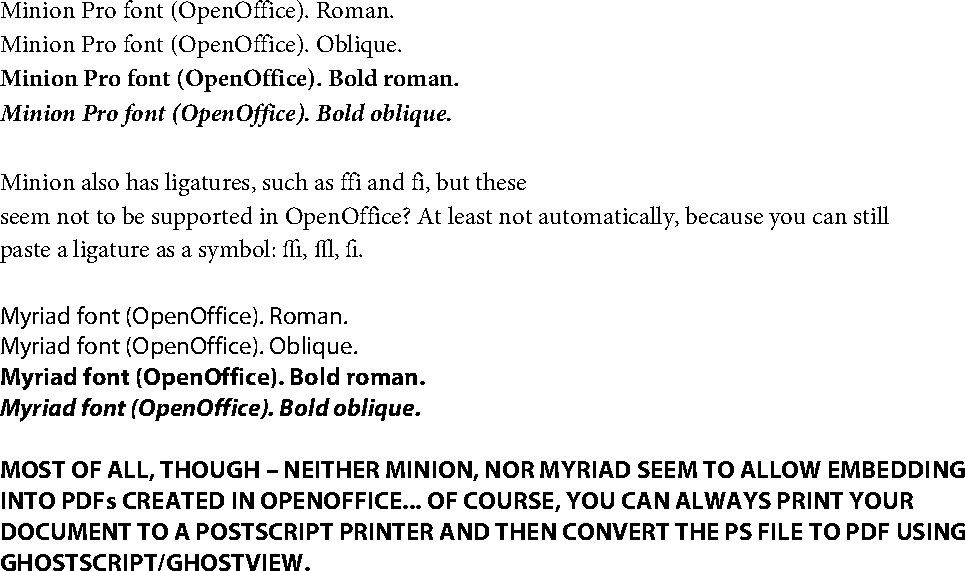
\includegraphics[width=.8\linewidth]{figures/openoffice}}
\caption{Myriad and Minion in OpenOffice. Support for ligatures sucks.}\label{fig:openoffice}
\end{figure}

\section{Making the fonts available to \LaTeX}

So far I've been working on a Windows box, so I'll go on with font installation on Mik\TeX{} and
we'll see if they work properly. We'll need packages \texttt{minionpro} and \texttt{mnsymbol} 
from CTAN. The first one is at:
\begin{center}\small
\url{http://www.tug.org/tex-archive/help/Catalogue/entries/minionpro.html}
\end{center}

Now, the procedure to install fonts goes like this, supposedly:
\begin{itemize}
    \item Install \texttt{mnsymbol} using Mik\TeX{} or manually.
    \item Unzip \texttt{minionpro} and follow instructions in the \texttt{README}
    file. LCDF Typetools project is at \url{http://www.lcdf.org/type/}, you'll need
    to install it first and add the \texttt{bin} folder to \texttt{PATH}. I followed
    the installation instructions almost exactly. The difference was that Mik\TeX\ requires
    a local \texttt{updmap.cfg} file (create it in:\\
    \texttt{localtexmf/miktex/config/updmap.cfg} \\
    and refresh the database with \texttt{initexmf --mkmaps}).

    \item Surprisingly, everything worked just as expected (see Figure~\ref{fig:minion}).
\end{itemize}

\begin{figure}[p]
\centering%
\fbox{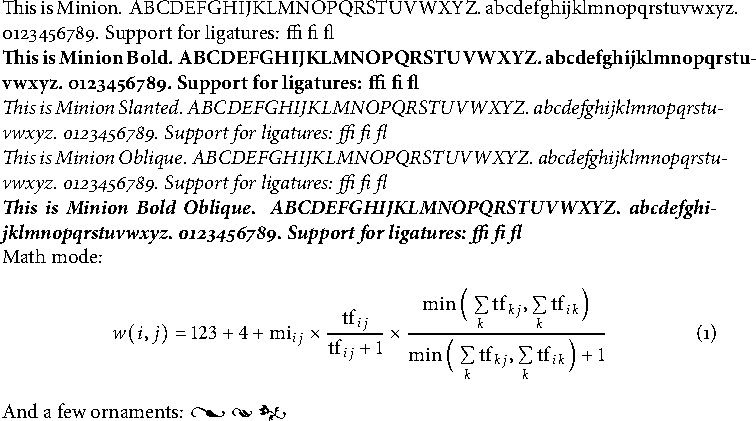
\includegraphics[width=.8\linewidth]{figures/minion-test}}
\caption{Minion in \LaTeX{}. Support for ligatures and text figures works as expected.}\label{fig:minion}
\end{figure}

\section{Whining}

Now it's time to whine a bit. I managed to get Minion working, but Myriad was beyond my current
time limits -- it'd require fiddling with \emph{fontools} and I've never done it before.

Another thing is the support for glyphs such as \textsc{Caps}, which are emulated if you only
have the four basic fonts. Not a perfect solution. 


\end{document}